\documentclass[times, utf8, seminar]{fer}
\usepackage{booktabs}
\usepackage{booktabs}
\usepackage{pdfpages}
\usepackage{braket}
\usepackage[inkscapeformat=png]{svg}
\usepackage{subcaption}
\usepackage[qm]{qcircuit}
\usepackage{graphicx}
\usepackage[noend]{algpseudocode}
\usepackage{algorithm}
\usepackage{amsmath}
\usepackage{amssymb}
\usepackage{listings}
\usepackage{makecell}
\usepackage{tabularx}
\usepackage{cellspace}
\usepackage{graphicx}
\usepackage{array, tabularx, caption, boldline}
\usepackage{framed}

\usepackage{courier}
\usepackage{url}
\usepackage[pdfa, hidelinks]{hyperref}

\def\UrlBreaks{\do\/\do-}
\setcitestyle{numbers,square,super}
\hypersetup{
	citecolor=black
}

\begin{document}
	
	% TODO: Navedite naslov rada.
	\title{Algoritam majmuna i algoritam krijesnica}
	
	% TODO: Navedite svoje ime i prezime.
	\author{Velimir Kovačić}
	
	% TODO: Navedite ime i prezime mentora.
	\voditelj{Marin Golub}
	
	\maketitle
	
	\tableofcontents
	
	\chapter{Uvod}
	Metaheuristika se odnosi na oblikovni obrazac koji ugrađuje prethodno znanje u izgradnju raznih optimizacijskih algoritama. Smatra se potpodručje stohastičke optimizacije. Stohastička optimizacija je kombinacija algoritama i slučajnih procesa radi pronalaženja optimalnih rješenja. 

Prirodom nadahnute metaheuristike su one koje crpe ideje za pretraživanje prostora stanja iz prirode. Algoritmi rojeva su potkategorija prirodno nadahnutih metaheuristika koji su nadahnuti kolektivnim ponašanjem životinja ili kukaca. Roj se sastoji od više individua čije je ponašanje vrlo jednostavno, ali zajedno mogu djelovati inteligentno. 

Postoje mnogi takvi algoritmi, najpoznatiji su mravlji algoritam i algoritam pčela. U ovom seminaru razmotrit će se manje poznati algoritam majmuna i algoritam krijesnica.

	\chapter{Algoritam majmuna}
	
\section{Uvod}
Algoritam majmuna \cite{ZHAOMA}  metaheuristički je optimizacijski algoritam utemeljen na načinu na koji se majmuni u prirodi penju na planine. Razvijen je za učinkovitu globalnu optimizaciju multimodalnih optimizacijskih problema  s kontinuiranim varijablama u visokim dimenzijama. 
\par
Funkcija cilja optimizacijskog problema može se zamisliti kao polje s planinama. Kako bi majmun pronašao najviši vrh u polju, izvodi 3 radnje:
\begin{enumerate}
	\item Penjanje 
	
	\item Gledanje i skakanje
	
	\item Salto
\end{enumerate}

Majmun se sa svoje početne točke penje uz planinu (Penjanje). U jednom trenutku staje, gleda oko sebe kako bi našao višu planinu i ako takva postoji, skače na nju (Gledanje i skakanje). Ponovno se penje uz planinu (Penjanje). Kako bi pronašli još višu planinu, mogu napraviti salto u novu domenu pretraživanja (Salto). Nakon što cijela populacija majmuna izvrši ovaj postupak dovoljno puta, dobije se izlaz algoritma koji je najviša točka koju su majmuni posjetili.

\par

U multimodalnim optimizacijskim problemima, broj lokalnih optimuma raste eksponencijalno s povećanjem dimenzije. Cilj salta u algoritmu je izbjegavanje prekomjernog lokalnog pretraživanja. Penjanje, koje ustvari je lokalno pretraživanje, koristi pseudogradijent koji se uvijek računa na temelju vrijednosti funkcije cilja za 2 točke (neovisno o dimenziji). To omogućava učinkovitiju optimizaciju u optimizacijskih problemima u visokim dimenzijama.

\section{Algoritam}
Algoritam prati opisani iterativni postupak penjanja majmuna dok se ne dosegne određeni broj iteracija $N$. Izlaz je položaj za koji je zabilježena najveća vrijednost funkcije cilja.

\begin{algorithm}
	\begin{algorithmic}[1]
		\Function{MA}{M, n, N, Nc, a, b, [c, d]}
		\State x = \Call{Postavljanje}{M, n}
		\State x* = x[0] 
		\For{iter = 1 to N}
		\State \Call{Penjanje}{Nc, x, x*, a}
		\State \Call{GledanjeSkakanje}{x, b}
		\State \Call{Penjanje}{Nc, x, x*, a}
		\State \Call{Salto}{x, [c, d]}
		\EndFor
		\State
		\Return x*
		\EndFunction
	\end{algorithmic}
	\caption{Algoritam majmuna}
\end{algorithm}



\subsection{Postavljanje početnih položaja}
Položaj majmuna predstavlja $n$-dimenzionalni vektor:
\begin{equation}
	\vec{x} = (x_1, x_2, \dots, x_n)
\end{equation}
Položaj $i$-tog od $M$ majmuna:
\begin{equation}
	\vec{x}_i = (x_{i1}, x_{i2}, \dots, x_{in})
\end{equation}

Na početku je potrebno postaviti početne položaje svih $M$ majmuna. Najjednostavnije je odrediti $n$-dimenzionalnu hiperkocku i iz nje uniformno uzorkovati položaj za svakog majmuna. Ako pojedini uzorkovani položaj ne zadovoljava ograničenja optimizacijskog problema, uzorkuje se ponovno dok ograničenja ne budu zadovoljena. Primjerice za hiperkocku $[0, 10]^{n}$:
\begin{algorithm}[H]
	\begin{algorithmic}[1]
		\Function{Postavljanje}{M, n}
		\State x = []
		\For{i = 1 to M}
		\Repeat
		\For{j = 1 to n}
		\State x[i][j] = rand(0, 10)
		\EndFor
		\Until{x[i] zadovoljava ograničenja}
		\EndFor
		\State
		\Return x
		\EndFunction
	\end{algorithmic}
	\caption{Postavljanje početnih položaja}
\end{algorithm} 

\subsection{Penjanje}
Cilj penjanja je doći do položaja za koji je funkcija cilja veća nego za trenutni. Za pomicanje koristi se pseudogradijent utemeljen na SPSA (\textit{simultaneous perturbation stochastic approximation}.)

\begin{enumerate}
	\item Za majmuna $i$ generira se vektor $\Delta\vec{x}_i = (\Delta\vec{x}_{i1}, \Delta\vec{x}_{i2}, \dots, \Delta\vec{x}_{in})$  gdje je
	\subitem  $\Delta\vec{x}_{ij} =
	\begin{cases}
		a & \text{s vjerojatnošću } 0.5 \\
		-a & \text{s vjerojatnošću } 0.5 \\
	\end{cases}$
	\subitem Parametar $a > 0$ zove se \textit{dužina koraka} i ovisi o optimizacijskom problemu.
	
	\item Računa se pseudogradijent funkcije cilja na položaju majmuna:
	\subitem $f'_i(\vec{x}_i) = (f'_{i1}(\vec{x}_i), f'_{i2}(\vec{x}_i), \dots, f'_{in}(\vec{x}_i))$ 
	
	\subitem $f'_{ij}(\vec{x}_i) = \frac{f(\vec{x}_i + \Delta\vec{x}_i) - f(\vec{x}_i - \Delta\vec{x}_i)}{2\Delta x_{ij}}$
	
	\item Neka je $\vec{y} = (y_1, y_2, \dots, y_n)$ gdje je
	\subitem $y_j = x_{ij} + a\cdot \text{sgn}(f'_{ij}(\vec{x}_i))$
	
	\item Ako $\vec{y}$ zadovoljava ograničenja, ažurira se položaj majmuna $\vec{x}_i \leftarrow \vec{y}$
\end{enumerate}

Za svakog majmuna se koraci 1 - 4 ponavljaju sve dok promjena funkcije cilja nije dovoljno mala ili dok se ne prođe maksimalan broj ponavljanja.

\begin{algorithm}[H]
	\begin{algorithmic}[1]
		\Function{Penjanje}{Nc, x, x*, a}
		\For{i = 1 to M}
		\Repeat
		\State $\Delta$x = []
		\State f' = []
		\State y = []
		\For{j = 1 to n}
		\State $\Delta$x[j] = rand([a, -a], [0.5, 0.5])
		\EndFor
		\For{j = 1 to n}
		\State f'[j] = (f(x[i] + $\Delta$x) - f(x[i] - $\Delta$x))/(2$\Delta$x[j])
		\EndFor
		\For{j = 1 to n}
		\State y[j] = x[i][j] + a*sgn(f'[j])
		\EndFor
		\If{y zadovoljava ograničenja} x[i] = y
		\EndIf
		\If{f(x[i]) > f(x*)} x* = x[i]
		\EndIf
		\Until{razlika f(x[i]) dovoljno mala ili dosegnut broj ponavljanja Nc}
		\EndFor
		\EndFunction
	\end{algorithmic}
	\caption{Penjanje}
\end{algorithm}



\subsection{Gledanje i skakanje}
Cilj gledanja i skakanja je prebaciti se na položaj u blizini čija je vrijednost funkcije cilja veća nego za trenutni. Definiran je parametar $b$ koji označava doseg majmunovog pogleda.

\begin{enumerate}
	\item Neka je $\vec{y} = (y_1, y_2, \dots, y_n)$ gdje je
	\subitem $y_j$ uzorkovan iz uniformne distribucije na $[x_{ij} - b, x_{ij} + b]$.
	
	\item Ako $\vec{y}$ zadovoljava ograničenja i vrijedi $f(\vec{y}) \ge f(\vec{x}_i)$, ažurira se položaj majmuna $\vec{x}_i \leftarrow \vec{y}$
\end{enumerate}

Za svakog majmuna se korak 1 ponavlja sve dok se ne zadovolji uvjet u koraku 2.

\begin{algorithm}[H]
	\begin{algorithmic}[1]
		\Function{GledanjeSkakanje}{x, b}
		\For{i = 1 to M}
		\Repeat
		\State y = []
		\For{j = 1 to n}
		\State y[j] = rand(x[i][j] - b, x[i][j] + b))
		\EndFor
		\Until{y zadovoljava ograničenja i f(y) >= f(x[i])}
		\State x[i] = y
		\EndFor
		\EndFunction
	\end{algorithmic}
	\caption{Gledanje i skakanje}
\end{algorithm}


\subsection{Salto}
Cilj salta je prebaciti se u novu domenu. Određuje se centroid položaja svih majmuna i svaki majmun radi salto u njegovom smjeru. Definiran je raspon $[c, d]$ iz kojeg se uniformno uzorkuje duljina salta.

Računa se centroid $p$:

\begin{equation}
	\vec{p} = \frac{1}{M} \sum_{i = 1}^{M} \vec{x}_i
\end{equation}

\begin{enumerate}
	
	\item Neka je $\vec{y} = \vec{x}_i + \alpha(\vec{p} - \vec{x}_i)$ gdje je
	\subitem $\alpha$ uzorkovan iz uniformne distribucije na $[c, d]$
	
	\item Ako $\vec{y}$ zadovoljava ograničenja, ažurira se položaj majmuna $\vec{x}_i \leftarrow \vec{y}$
\end{enumerate}

Za svakog majmuna se korak 1 ponavlja sve dok se ne zadovolji uvjet u koraku 2.

\begin{algorithm}[H]
	\begin{algorithmic}[1]
		\Function{Salto}{x, [c, d]}
		
		\State p = []
		
		\For{i = 1 to M}
		\State p += x[i]
		\EndFor
		
		\State p = p/M
		
		\For{i = 1 to M}
		\Repeat
		\State $\alpha$ = rand(c, d)
		\State y = x + $\alpha$ * (p - x[i])
		
		\Until{y zadovoljava ograničenja}
		\State x[i] = y
		\EndFor
		\EndFunction
	\end{algorithmic}
	\caption{Salto}
\end{algorithm}



\section{Programsko ostvarenje}
\subsection{Primjer funkcije za maksimizaciju}
Neka se maksimizira $n$-dimenzionalna funkcija:
\begin{align*}
	&f(\vec{x}) = -(\vec{x}^\intercal\vec{x}) \label{eq:fx} \tag{4.4} \\
	&\vec{x} \in [-100, 100]^n
\end{align*}
Funkcija ima maksimum u točki $\vec{0}$ i on iznosi $f(\vec{0}) = 0$. Minimum je na kutovima domene i iznosi $-100^2n$.

\begin{figure}[H]
	\centering
	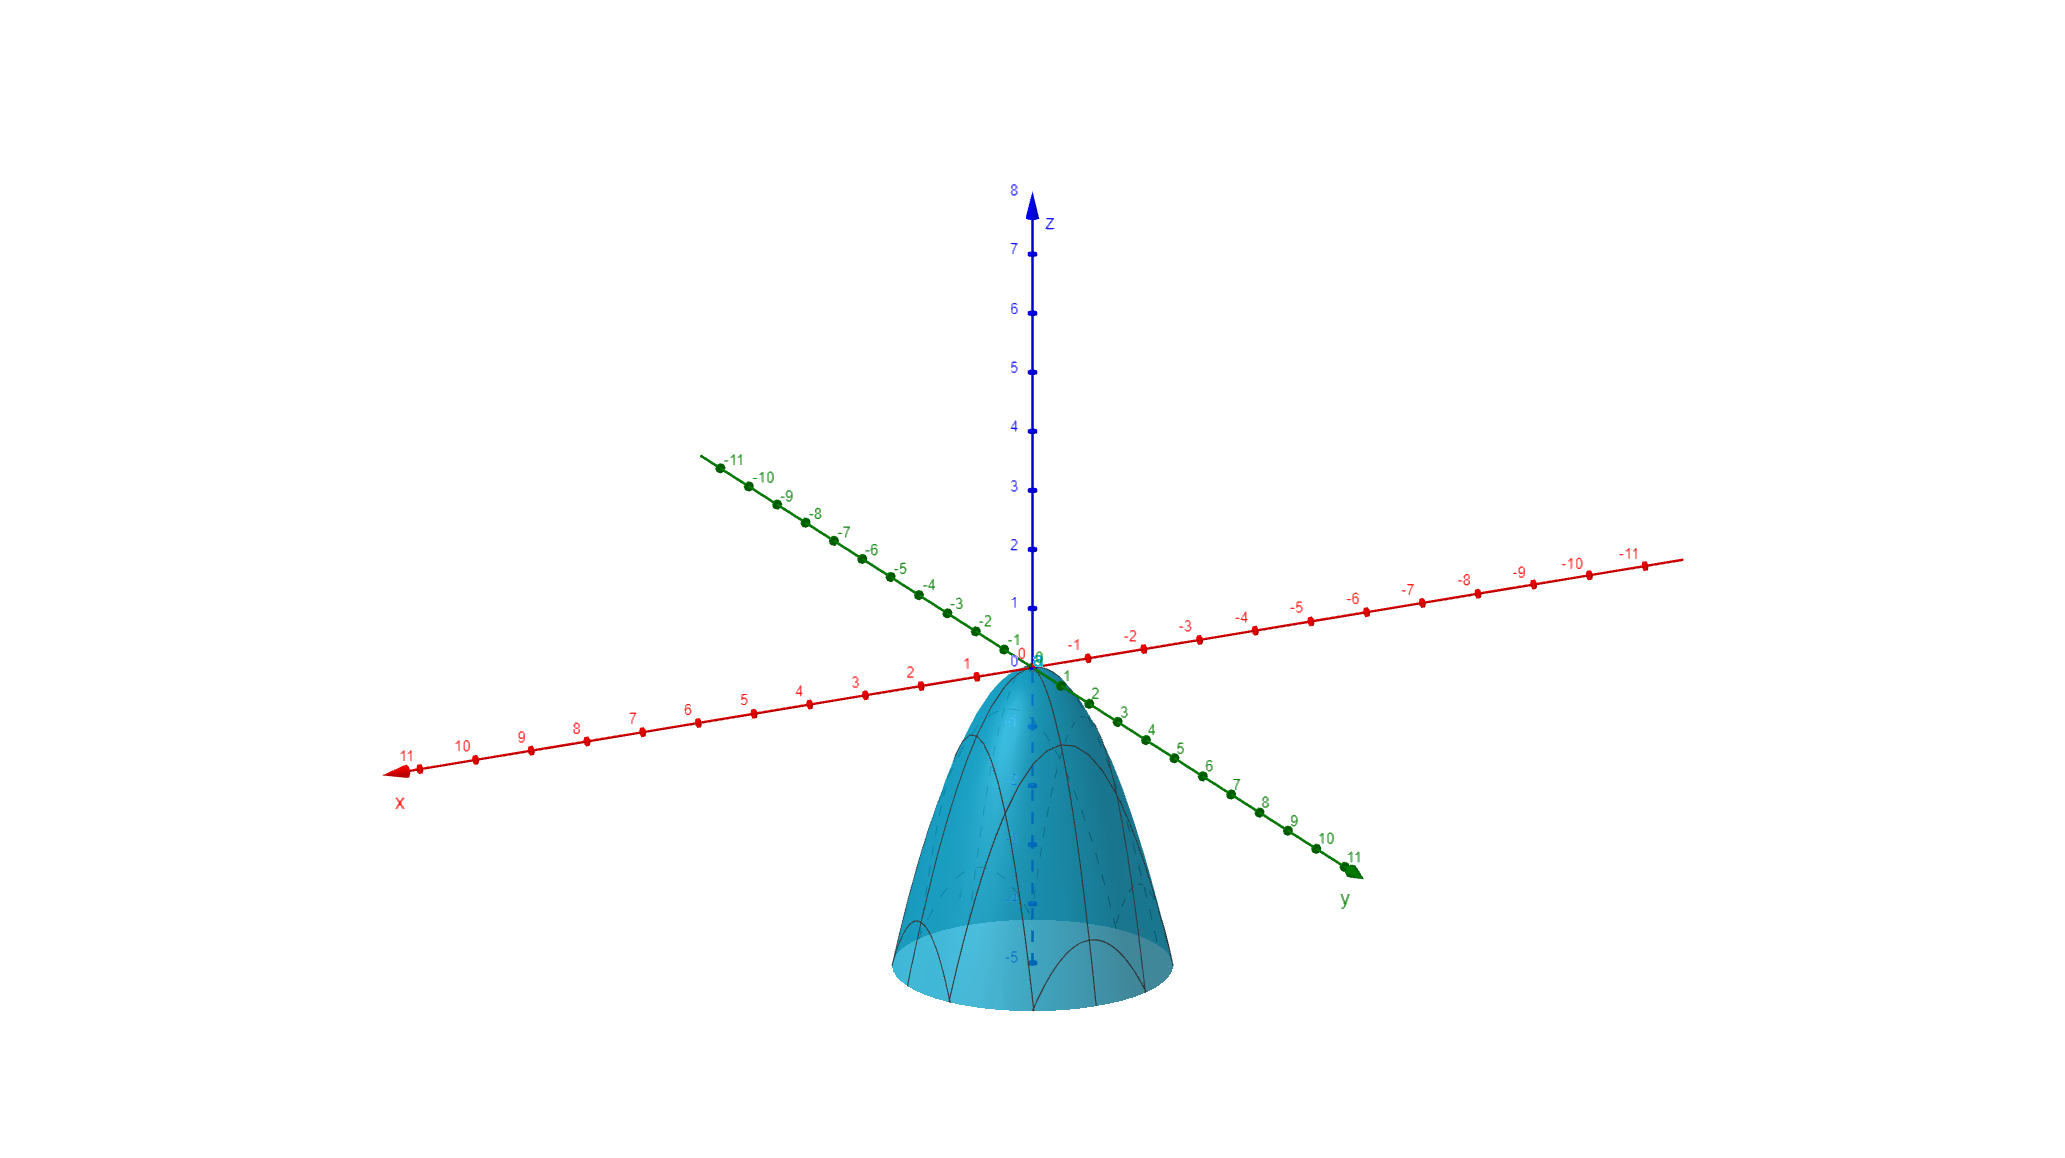
\includegraphics[width=14cm]{geogebra}
	\caption{Graf funkcije $f(\vec{x})$ za $n = 2$} 
	
\end{figure}

\subsection{Vlastito programsko ostvarenje}
Vlastito programsko ostvarenje algoritma majmuna povedeno je prevođenjem pseudokoda u programski jezik Python. Korištene su knjižnice programa za Python: \textit{numpy} i \textit{random}. Sastoji od klase \verb|MA| sa sljedećim metodama:

\begin{enumerate}
	\item \verb|__init__(self, M, N, Nc, a, b, c, d)|
	
	Instanciranje klase i postavljanje parametara algoritma
	
	
	\item \verb|optimize(self, f, cond, n, l, r)| 
	
	Optimizacija funkcije \verb|f| s funkcijom ograničenja \verb|cond|
	
	\item \verb|initialize(self, cond, l, r, M, n)| 
	
	Generiranje početnih položaja svih majmuna
	
	\item \verb|climb(self, M, Nc, n, X, a)| 
	
	
	\item \verb|watchJump(self, M, n, X, b)| 
	
	
	\item \verb|sumersault(self, M, n, X, c, d)| 
	
	
	\item Pomoćne funkcije:
	
	\subitem \verb|sampleHypercube(self, n, l, r)| 
	
	
	\subitem \verb|sampleWatch(self, n, x, b)| 
	
	\subitem \verb|sampleDx(self, n, a)| 
	
\end{enumerate}

\begin{tabular}{|m{1cm}|m{11cm}|}
	
	\hline
	\verb|M| & Broj majmuna \\
	\hline
	\verb|N| & Broj iteracija algoritma \\
	\hline
	\verb|Nc| & Broj skakanja \\
	\hline
	\verb|f| & Funkcija koja se optimira \\
	\hline
	\verb|cond| & Funkcija kojom se provjerava zadovoljenost ograničenja \\
	\hline
	\verb|n| & Dimenzionalnost ulaza funkcije \\
	\hline
	\verb|a| & Duljina skoka \\
	\hline
	\verb|b| & Udaljenost pogleda \\
	\hline
	\verb|c| & Donja granica duljine salta \\
	\hline
	\verb|d| & Gornja granica duljine salta \\
	\hline
	\verb|l| & Donja granica u svakoj dimenziji hiperkocke  \\
	\hline
	\verb|r| & Donja granica u svakoj dimenziji hiperkocke \\
	\hline
	\verb|X| & Lista svih majmuna \\
	\hline
	\verb|x| & Položaj pojedinog majmuna \\
	\hline
\end{tabular}


Na primjer, optimira se funkcija \eqref{eq:fx} s $n = 30$ dimenzija koristeći $M = 5$ majmuna, $N = 60$ iteracija, $Nc = 500$ skokova, duljinom koraka $a = 0.0001$, udaljenošću pogleda $b = 10$ i duljinom salta $[c, d] = [-1, 1]$.

Klasa \verb|MA| nalazi se u datoteci \verb|ma.py|. Može se pokrenuti na sljedeći način:


\begin{framed}
	\begin{verbatim}import ma
		import numpy as np
		import matplotlib.pyplot as plt
		
		f = lambda x : -np.dot(x, x)
		cond=lambda x : np.max(x) < 100 and np.min(x) > -100
		
		m = ma.MA(M=5, N=60, Nc=500, a=0.0001, b=10, c=-1, d=1)
		x, fs = m.optimize(f=f, cond=cond, n=30, l=-100, r=100)
		
		print("x* =", x)
		print("f(x*) =", f(x))
		
		plt.plot(range(1, len(fs)), fs[1:])
		plt.show()
	\end{verbatim}
\end{framed}

\noindent Izlaz ovog primjera je:
\begin{framed}
	\begin{verbatim}
		x* = [ 3.29615006  4.05143309  ...  -3.15835887]
		f(x*) = -330.1389091136464
	\end{verbatim}
\end{framed}

\begin{figure}[h]
	\centering
	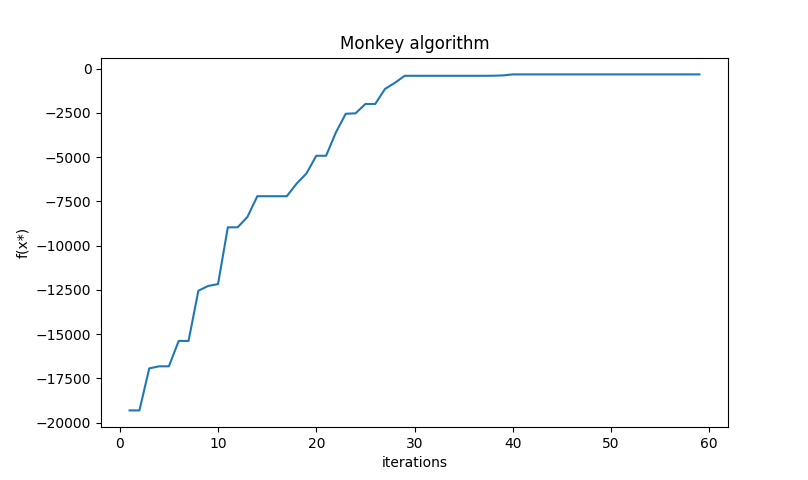
\includegraphics[width=14cm]{Figure_1}
	\caption{Graf ovisnosti izlaza funkcije o broju iteracija za dani primjer} 
	
\end{figure}



\subsection{Programsko ostvarenje MQL5}
\label{sec:mql5majmun}
Programsko ostvarenje algoritma majmuna autora A. Dika\cite{DIKMA} može se preuzeti na internetskoj stranici \href{https://www.mql5.com/en/articles/12212}{MQL5}. Važno je napomenuti da se ovo ostvarenje razlikuje se od onog u pseudokodu u pogledu funkcija \textit{gledanje i skakanje} i \textit{salto}.

Za pokretanje potrebno je instalirati program \href{https://www.metatrader5.com/en}{Meta Trader 5}, otvoriti korisnički račun i unutar programa otvoriti dijagram za proizvoljni \textit{symbol}. Zip dokument s algoritmima smjesti se u podatkovnu strukturu programa MQL5.


 Za pokretanje algoritma na preddefiniranim testnim funkcijama odabire se \verb|Scripts/Test_OA_MA.mq5| u \textit{Navigatoru}. U novootvorenom prozoru postavljaju se parametri i pokreće se algoritam koji u stvarnom vremenu prikazuje položaje majmuna na hiperravnini i ispisuje rezultat i pogrešku. 

\begin{figure}[H]
	\centering
	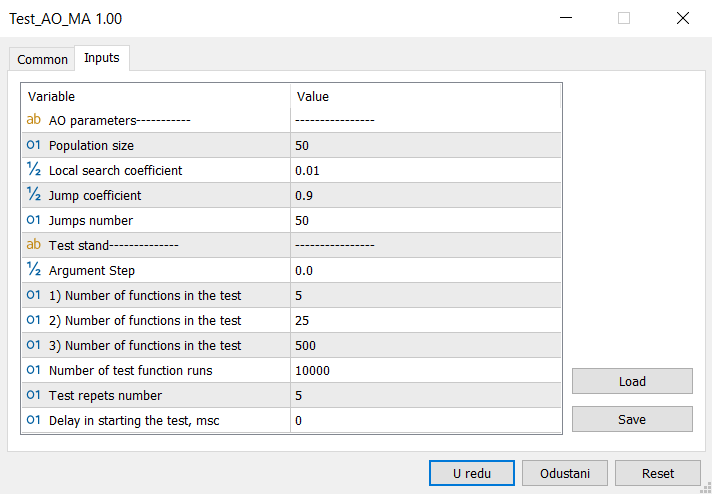
\includegraphics[width=14cm]{mt51}
	\caption{Odabir parametara algoritma u Meta Traderu 5} 
	
\end{figure}

\begin{figure}[H]
	\centering
	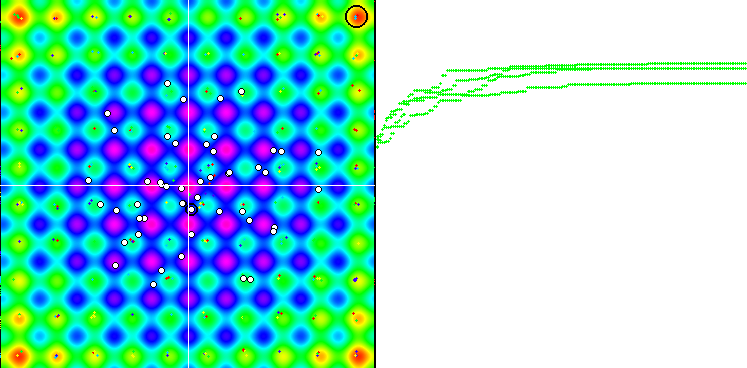
\includegraphics[width=14cm]{mt52}
	\caption{Položaji majmuna (bijele točke) u stvarnom vremenu na hiperravnini (lijevo) i izlazi funkcije cilja za 4 pokretanja algoritma (desno)}
	\centering
	
\end{figure}

\noindent Ispis je:
\begin{framed}
	\begin{verbatim}
		5 Rastrigin's; Func runs 10000 result: 68.03668259
		Score: 0.84301
		25 Rastrigin's; Func runs 10000 result: 55.4356683739
		Score: 0.68688
		500 Rastrigin's; Func runs 10000 result: 41.238597562
		Score: 0.51097
		=============================
		5 Forest's; Func runs 10000 result: 0.445023241351
		Score: 0.25173
		25 Forest's; Func runs 10000 result: 0.183789574445
		Score: 0.10396
		500 Forest's; Func runs 10000 result: 0.062930759789
		Score: 0.03560
		=============================
		5 Megacity's; Func runs 10000 result: 2.63999999999
		Score: 0.22000
		25 Megacity's; Func runs 10000 result: 1.11199999999
		Score: 0.09267
		500 Megacity's; Func runs 10000 result: 0.3276
		Score: 0.02730
	\end{verbatim}
\end{framed}

Vlastite funkcije za optimizaciju definiraju se u \verb|Include/Math/functions.mqh| u programskom jeziku temeljenom na C++. Funkcija \eqref{eq:fx} može se definirati na sljedeći način:

\begin{framed}
	\begin{verbatim}
		class C_Sphere : public C_Function
		{
			public: //====================================
			C_Sphere ()
			{
				SetNamFun ("Sphere");
				
				SetMinX (-100.0);
				SetMaxX ( 100.0);
				SetMinY (-100.0);
				SetMaxY ( 100.0);
				
				SetMinFun   (-20000.0);       //4 points
				SetMinFuncX (100.0);
				SetMinFuncY (100.0);
				
				SetMaxFun   (0.0);           //1 points
				SetMaxFuncX (0.0);
				SetMaxFuncY (0.0);
			}
			
			private: //===================================
			double Core (double x, double y)
			{
				double res = -(x*x + y*y);
				return(res);
			}
		};
	\end{verbatim}
\end{framed}

Za pokretanje optimizacije proizvoljne funkcije, potrebno je u \verb|Test_OA_MA.mq5| u funkciji \verb|void OnStart()| upisati poziv funkcije \verb|FuncTests|. Parametri funkcije su: funkcija, dimenzija $n/2$ i boja linije na grafu funkcije cilja. Primjerice za funkciju \verb|C_Sphere|:

\begin{framed}
	\begin{verbatim}
		C_Sphere F;
		FuncTests(F, 15, clrLime);
	\end{verbatim}
\end{framed}


Optimira se funkcija \eqref{eq:fx} s  $n = 30$ dimenzija s $M = 50$ majmuna, $N = 50000$ iteracija, $Nc = 50$ skokova, duljinom koraka $a = 0.01$ i udaljenošću pogleda $b = 0.9$.


\begin{figure}[H]
	\centering
	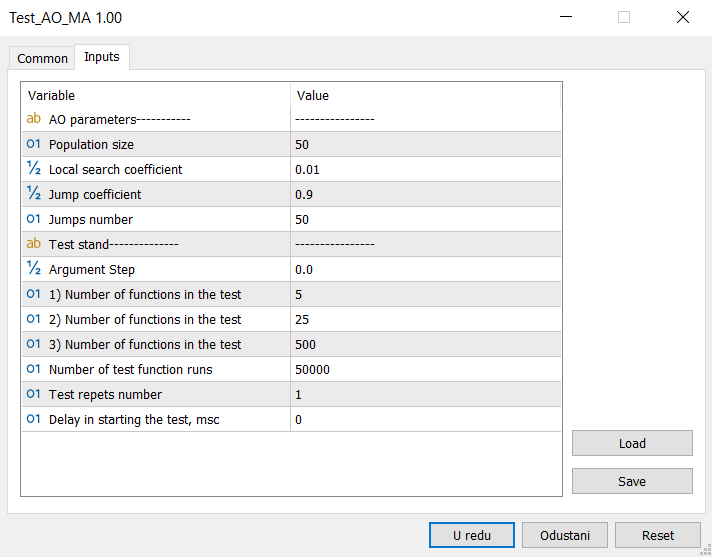
\includegraphics[width=14cm]{mt53}
	\caption{Odabir parametara algoritma za primjer}
	\centering
\end{figure}

\begin{figure}[H]
	\centering
	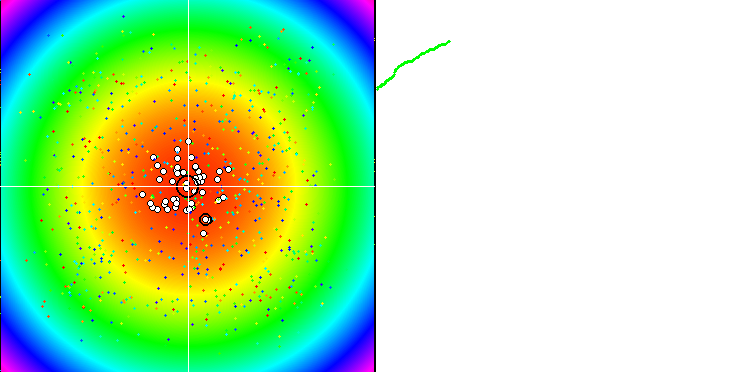
\includegraphics[width=14cm]{mt54}
	\caption{Položaji majmuna na hiperravnini i izlazi funkcije cilja tijekom izvođenja}
	\centering
\end{figure}

\begin{figure}[H]
	\centering
	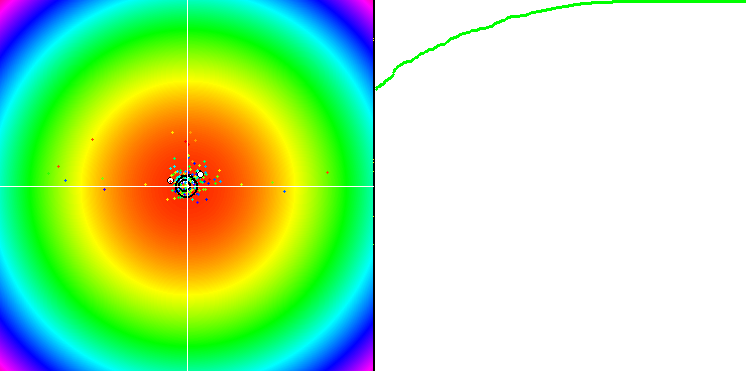
\includegraphics[width=14cm]{mt55}
	\caption{Položaji majmuna na hiperravnini i izlazi funkcije cilja nakon izvođenja}
	\centering
\end{figure}

\noindent Ispis je:
\begin{framed}
	\begin{verbatim}
		15 Sphere's; Func runs 50000 result: -2.5525976674831137
		Score: 0.99987
	\end{verbatim}
\end{framed}








\section{Primjene}

\subsection{Optimizacija hibridnih mikromreža}
Izmijenjeni algoritam majmuna upotrebljen je za optimizaciju konfiguracije komponenti hibridnih mikromreža.\cite{ITUARTEVILLARREAL2012344} Minimizirana je cijena i emisija stakleničkih plinova. Algoritam je izmijenjen uvođenjem meteoroloških faktora.


\subsection{Grupiranje}
Hibridni algoritam majmuna utemeljen na operatoru pretraživanja iz algoritma kolonije pčela upotrebljen je za grupiranje. \cite{Chen2014} Pokazano je da ima dobre performanse na sintetičkim i stvarnim skupovima podataka.

\subsection{0-1 problem naprtnjače}
Izmijenjenim algoritam majmuna predložen je za rješavanje 0-1 problema naprtnjače.\cite{ZHOU2016817} Lokalno pretraživanje ojačano je pohlepnima algoritmom a salto je izmijenjen kako bi se izbjeglo upadanje u lokalne optimume. Uveden je i kooperativni proces radi ubrzanje konvergencije. Pokazano je da je izmijenjeni algoritam majmuna učinkovita alternativa za rješavanje ovog problema.

\subsection{Raspoređivanje zadataka u računarstvu u oblaku}
Algoritam majmuna primijenjen je na raspoređivanje zadataka u računarstvu u oblaku.\cite{8313789} Minimizirana je cijena i maksimizirana iskorištenost kako bi se pružila bolja usluga klijentu. Pokazano je da takav algoritam radi učinkovitije od prethodno predloženih.

\subsection{Flow-shop scheduling}
Za NP-teški kombinatorni problem \textit{flow-shop scheduling} upotrebljen je hibridni algoritam majmuna s pod-populacijama.\cite{MARICHELVAM201782} Algoritam majmuna nadmašio je mnoge heurističke i metaheurističke algoritme iz literature.

\subsection{Raspoređivanje elektroničkih komponenata u računalima}
Algoritam majmuna korišten je za optimiziranje problema raspoređivanja elektroničkih komponenata u računalima.\cite{Kuliev_2018} Pokazano je da daje učinkovitija rješenja nego genetski algoritam.

\subsection{Set cover problem}
Za rješavanje \textit{set cover} problema, dizajniran je binarni algoritam majmuna.\cite{Crawford2020} Izmijenjen je proces penjanja majmuna i dodan je proces kooperacije. Pokazuje se da takav algoritam nadmašuje mnoge heurističke i metaheurističke algoritme iz literature. 


\subsection{Prepoznavanje tumora u MRI slikama mozga}
Automatizirani algoritam majmuna korišten je pronalaženje i segmentaciju lokacija tumora na MRI slikama mozga.\cite{Alagarsamy_2020} Tehniku je moguće upotrijebiti za pomoć radiolozima pri pronalaženju tumora.

	
	\chapter{Algoritam krijesnica}
	\section{Uvod}
Algoritam krijesnica\cite{10.1007/978-3-642-04944-6_14} metaheuristički je optimizacijski algoritam sličan algoritmu rojeva čestica. Nadahnut je načinom na koji se krijesnice u prirodi međusobno privlače. 

Krijesnice imaju sposobnost međusobnog odašiljanja svjetlosnih signala svojim svjetlećim organima. Neke vrste odašilju trepteće, a neke konstanto svjetlo. Takvi signali služe za privlačenje partnera za parenje i privlačenje potencijalnog plijena. U nekim vrstama mužjaci privlače ženke, a u drugima obratno.


\section{Algoritam}
U samom algoritmu razmatramo međusobno privlačenje krijesnica. Potrebno je idealizirati svojstva svijetljenja:

\begin{enumerate}
	\item Ne razlikujemo muške i ženske krijesnice, sve svijetle i sve se međusobno privlače.
	\item Privlačnost je proporcionalna intenzitetu svjetla kojeg odašilju i opada kvadratom udaljenosti $I \propto \frac{1}{r^2}$. Ona krijesnica s većim intenzitetom svjetla privlači onu s manjim.
	\item Intenzitet svjetla krijesnice određen je funkcijom cilja.
\end{enumerate}



\subsection{Privlačnost}
Za intenzitet svjetla same krijesnice moguće je u najjednostavnijem slučaju uzeti $I_0(\vec{x}) \propto f(\vec{x})$ (za maksimizacijske probleme) ili $I_0(\vec{x}) \propto -f(\vec{x})$ (za minimizacijske probleme). Ključno je pitanje kakav intenzitet svjetla vide druge krijesnice, to jest koliku imaju privlačnost $\beta$.

Intenzitet svjetla na udaljenosti $r$ je:

\begin{equation}
	I(r) = \frac{I_0}{r^2}
\end{equation}

Apsorpcija svjetla okoline $\gamma$ je:

\begin{equation}
	I(r) = I_0 e^{-\gamma r}
\end{equation}

Ova dva izraza mogu se kombinirati u Gaussovoj formi čime se izbjegava nedefinirana vrijednost intenziteta svjetla na udaljenosti $r = 0$:

\begin{equation}
	I(r) = I_0 e^{-\gamma r^2}
\end{equation}

Mogu se upotrijebiti i druge monotono padajuće funkcije:

\begin{equation}
	I(r) = \frac{I_0}{1 + \gamma r^2}
\end{equation}

Kako se definirao intenzitet svjetlosti, tako se može definirati privlačnost:

\begin{equation}
	\beta(r) = \beta_0 e^{-\gamma r^2}
\end{equation}

Privlačnost se može definirati i kao bilo koja monotono padajuća funkcija oblika:

\begin{equation}
	\beta(r) = \beta_0 e^{-\gamma r^m}
\end{equation}


Karakteristična udaljenost $\Gamma$ je udaljenost na kojoj privlačnost opada s $\beta_0$ na $\beta_0e^{-1}$. Ona iznosi $\Gamma = \gamma^{\frac{-1}{m}}$. Isto tako, na temelju karakteristične udaljenosti nekog problema, može se odrediti konstanta apsorpcije svjetla $\gamma = \frac{1}{\Gamma^m}$

\subsection{Kretanje}
Položaj krijesnice predstavlja $n$-dimenzionalni vektor:
\begin{equation}
	\vec{x} = (x_1, x_2, \dots, x_n)
\end{equation}
Položaj $i$-te od $N$ krijesnica:
\begin{equation}
	\vec{x}_i = (x_{i1}, x_{i2}, \dots, x_{in})
\end{equation}
Udaljenost između krijesnica računamo euklidskom udaljenošću:
\begin{equation}
	r_{ij} = ||\vec{x}_i - \vec{x}_j|| = \sqrt{\sum_{k = 1}^{n}(x_{ik} - x_{jk})^2}
\end{equation} 
Kretanje krijesnice $i$ prema krijesnici $j$ većeg intenziteta svjetla je:
\begin{equation}
	\vec{x}_i \leftarrow \vec{x}_i + \beta_0e^{-\gamma r_{ij}^m}(\vec{x}_j - \vec{x}_i) + \alpha rand(-1, 1)
\end{equation}

Drugi pribrojnik predstavlja pomak u smjeru privlačne krijesnice, a treći predstavlja slučajni pomak. 

Uobičajeno je uzeti da su parametri $m = 2$, $\beta_0 = 1$ i $\alpha \in [0, 1]$. To ostavlja parametar $\gamma$ čiji odabir najviše utječe na konvergenciju algoritma, uobičajeno ga je odrediti na temelju karakteristične udaljenosti $\Gamma$.

\subsection{Pseudokod}

\begin{algorithm}[H]
	\begin{algorithmic}[1]
		\Function{FA}{n, N, maxGen, $\gamma$}
		
		\State X = \Call{Inicijalizacija}{n, d}
		\While{gen < maxGen}
		\For{i = 1 to n}
		\For{j = 1 to n}
		\If{I(X[j]) > I(X[i])} 
		\State Pomakni krijesnicu X[i] prema krijesnici X[j]
		\State Ažuriraj intenzitet svjetla krijesnice X[i]
		\EndIf
		\EndFor
		\EndFor
		\State Ažuriraj najbolje rješenje x*
		\EndWhile
		\State \Return x*	
		\EndFunction
	\end{algorithmic}
	\caption{Algoritam krijesnica}
\end{algorithm}

\section{Programsko ostvarenje}
\subsection{Programsko ostvarenje MEALPY}
Algoritam krijesnica i mnogi drugi metaheuristički algoritmi programski su ostvareni u sklopu knjižnice programa otvorenog koda \href{https://mealpy.readthedocs.io/en/latest}{MEALPY} programskog jezika Python. Knjižnica se može preuzeti naredbom konzole:


\begin{framed}
	\begin{verbatim}
		> pip install mealpy
	\end{verbatim}
\end{framed}

Prethodno opisani problem funkcije \eqref{eq:fx} s $n = 30$ definira se u programu kao rječnik i pokreće se algoritam krijesnica s 1000 epoha, brojem krijesnica $N = 50$,  $\gamma = 0.1$,  $\beta_0 = 1$, $\alpha = 0.5$ i $m = 2$:
\begin{framed}
	\begin{verbatim}
		import numpy as np
		from mealpy import FloatVar, FFA
		
		n = 30
		
		def objective_function(solution):
		return -np.sum(solution**2)
		
		problem = {
			"obj_func": objective_function,
			"bounds": FloatVar(lb=(-10., )*n, ub=(10., )*n),
			"minmax": "max",
		}
		
		
		model = FFA.OriginalFFA(epoch=1000, pop_size=50, 
		gamma = 0.1, beta_base = 1, 
		alpha = 0.5, exponent = 2)
		
		g_best = model.solve(problem)
		
		print("Solution:", g_best.solution)
		print("Fitness:", g_best.target.fitness)
	\end{verbatim}
\end{framed}


\noindent Izlaz ovog primjera je:
\begin{framed}
	\begin{verbatim}
		Solution: [-1.77332972  2.96553989 ...  -3.77894221]
		Fitness: -146.04412518749243
	\end{verbatim}
\end{framed}

\subsection{Programsko ostvarenje MQL5}
Programsko ostvarenje A. Dika u jeziku MQL5 može se preuzeti i pokrenuti na način analogan onom opisanom u odjeljku \ref{sec:mql5majmun}.

Primjer pokretanja \eqref{eq:fx} s $n = 30$ s 1000 epoha, $N = 50$,  $\gamma = 0.1$,  $\beta_0 = 1$, $\alpha = 0.5$:

\begin{figure}[H]
	\centering
	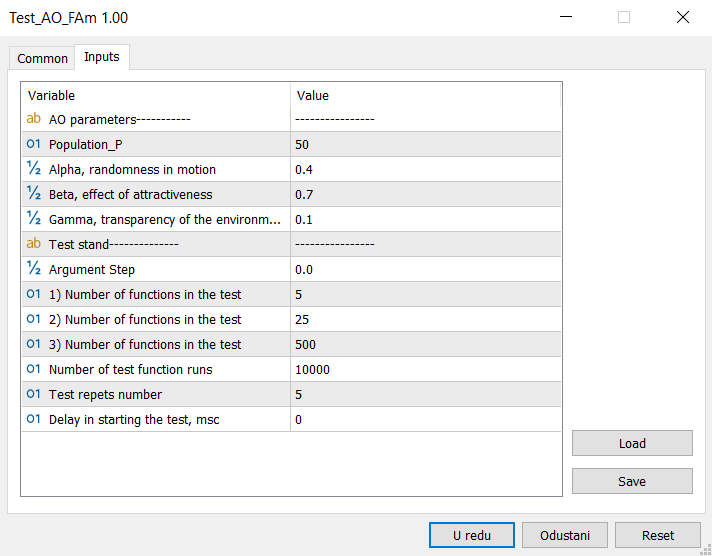
\includegraphics[width=14cm]{mt61}
	\caption{Odabir parametara algoritma za primjer}
	\centering
\end{figure}

\begin{figure}[H]
	\centering
	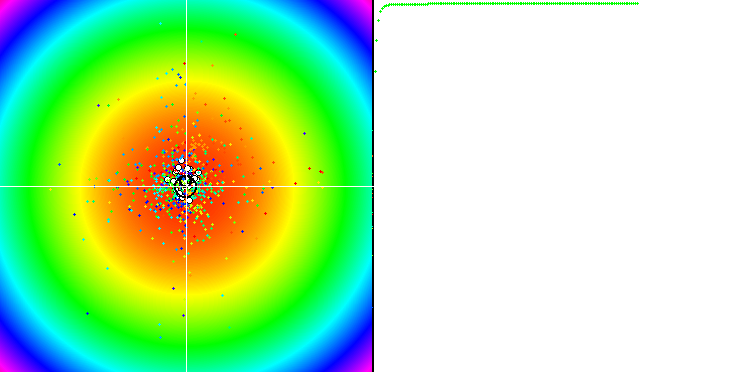
\includegraphics[width=14cm]{mt62}
	\caption{Položaji krijesnica na hiperravnini i izlazi funkcije cilja tijekom izvođenja}
	\centering
\end{figure}

\noindent Ispis je:
\begin{framed}
	\begin{verbatim}
		15 Sphere's; Func runs 10000 result: -70.09166510586255
		Score: 0.99650
	\end{verbatim}
\end{framed}



\section{Primjene}

\subsection{Economic Emissions Load Dispatch problem}
Algoritam krijesnica primijenjen je na problem \textit{Economic Emissions Load Dispatch} u kojem se istovremeno minimizira cijena i količina emisija stakleničkih plinova.\cite{Apostolopoulos2010} Pokazalo se da je uz pravilan odabir parametara moguće postići dobra rješenja.

\subsection{Kombinatorna optimizacija}
Hibridna inačica algoritma krijesnica, uz heuristiku lokalnog pretraživanja, upotrebljena je na problemu bojanja grafa s 3 boje.\cite{fister2012memetic} Rezultati su bili obećavajući i pokazali da je moguće koristiti algoritam i za druge kombinatorne probleme.


\subsection{Punjenje hladnjaka radi uštede energije}
Poboljšani algoritam krijesnica (IFA) korišten je za rješavanje problema punjenja hladnjaka.\cite{COELHO2013273} Imao je bolje performanse od nekoliko optimizacijskih algoritama iz literature.

\subsection{Segmentacija slika}
Algoritam krijesnica i algoritam $k$-NN korišteni su u kombinaciji za grupiranje piksela slika u $k$ grupa.\cite{7857598}

\subsection{Procjena potražnje vodenih resursa}
Novi dinamični algoritam krijesnica (NDFA) korišten je za procjenu potražnje vodenih resursa u gradu Nanchangu u Kini.\cite{WANG201895} Podaci o potražnji od 2003. do 2012. korišteni su za učenje modela, a predviđanje je ispitivano na podacima  od 2013. do 2015. Točnost predviđanja bila je $97.91\%$.

\subsection{Navigacija mobilnih robota u promjenjivim okolinama}
Navigacija grupe mobilnih robota u promjenjivim okolinama ostvarena je algoritmom krijesnica u kojem roboti predstavljaju krijesnice i vodeći se algoritmom, istražuju okolinu.\cite{PATLE2018691} Pokazalo se da su performanse ovog rješenja bolje nego drugih predloženih.

\subsection{Odabir značajki za detekciju upada na mrežma}
Algoritam krijesnica upotrebljen je za odabir značajki na temelju kojih se detektira upad.\cite{B2019148} Rezultat je pokazao je obećavajuć napredak u odnosu na druge prijedloge rješenja.

\subsection{Optimizacija životnog vijeka mreže bežičnih senzora}
Za optimizaciju životnog vijeka mreže bežičnih senzora korišten je poboljšani algoritam krijesnica (IFA).\cite{9148087} Simulacijama je pokazano da taj algoritam ima bolje i ujednačenije performanse od drugih algoritama.

	
	\chapter{Zaključak}
	Oba algoritma (algoritam majmuna i algoritam krijesnica) unatoč vrlo jednostavnim formulacijama pokazuju obećavajuće rezultate na stvarnim problemima od znanstvenih i matematičkih do industrijskih i komercijalnih. 

Općenito, prirodnom nadahnuti metaheuristički algoritmi rojeva na učinkovit način će pronaći neko rješenje problema. Takvo rješenje neće nužno biti najbolje moguće, ali može biti dovoljno dobro za pojedino područje primjene. Daljnjim istraživanjem mogu se pronaći učinkovitiji algoritmi i poboljšati postojeći.
	
	\bibliography{literatura}
	\bibliographystyle{fer}
	\nocite{*}
	
	\chapter{Sažetak}
	Algoritam majmuna i algoritam krijesnica metaheuristički su optimizacijski algoritmi rojeva. U ovom radu dan je pregled samih algoritama, načini na koje se mogu izvesti na računalu i njihove primjene.
	
\end{document}